

%%%%%%%%%%%%%%%%%%%%%%%%%%%%%%%%%%%%%%%%%%%%%%%%%%%%%%%%%%%%%%%%%%%%%%%%%
%%%%%%%%%%%%%%%%%%%%%%%%%%%%%%%%%%%%%%%%%%%%%%%%%%%%%%%%%%%%%%%%%%%%%%%%%
%%%%%%%%%%%%%%%%%%%%%%%%%%%%%%%%%%%%%%%%%%%%%%%%%%%%%%%%%%%%%%%%%%%%%%%%%

\begin{frame}{The influence function}

\begin{itemize}
    \item Weights as derivatives
    \item Influence function
    \item Simulation
    \item Experiments
\end{itemize}

\end{frame}

%%%%%%%%%%%%%%%%%%%%%%%%%%%%%%%%%%%%%%%%%%%%%%%%%%%%%%%%%%%%%%%%%%%%%%%%%
%%%%%%%%%%%%%%%%%%%%%%%%%%%%%%%%%%%%%%%%%%%%%%%%%%%%%%%%%%%%%%%%%%%%%%%%%
%%%%%%%%%%%%%%%%%%%%%%%%%%%%%%%%%%%%%%%%%%%%%%%%%%%%%%%%%%%%%%%%%%%%%%%%%


\begin{frame}{The linear approximation.}
%
%Suppose we have $N$ data points $\d_{1}, \ldots, \d_{N}$.  Then:
%
% \begin{align*}
% %
% \thetahat(\w) :=
% \vec\theta \,\, \textrm{ such that } \,\,
% \sumn
% \w_{n} G(\vec\theta, \d_{n}) =  \zP .
% %
% \end{align*}

\begin{minipage}{0.49\textwidth}
    \onslide<1-> {
    Original weights: \par
    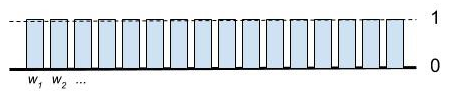
\includegraphics[width=0.68\textwidth]{static_figures/orig_weights}
    }
    \onslide<1-> {
    \par Leave-one-out weights: \par
    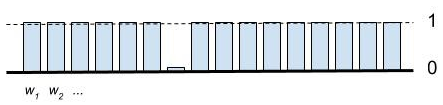
\includegraphics[width=0.68\textwidth]{static_figures/weights_loo}
    }
    \onslide<1-> {
    \par Bootstrap weights: \par
    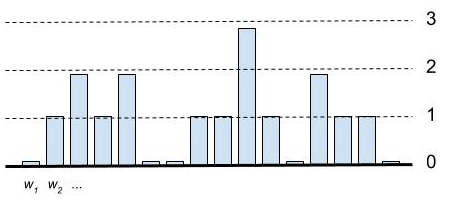
\includegraphics[width=0.68\textwidth]{static_figures/boot_weights}
    }
\end{minipage}
%\onslide<1->{
\begin{minipage}{0.49\textwidth}
    % https://www.overleaf.com/learn/latex/TikZ_package
    % https://latexdraw.com/how-to-annotate-an-image-in-latex/
    % https://tex.stackexchange.com/questions/9559/drawing-on-an-image-with-tikz
    \begin{tikzpicture}
        \onslide<1-> {
        \node[anchor=south west,inner sep=0] (image) at (0,0) {
            %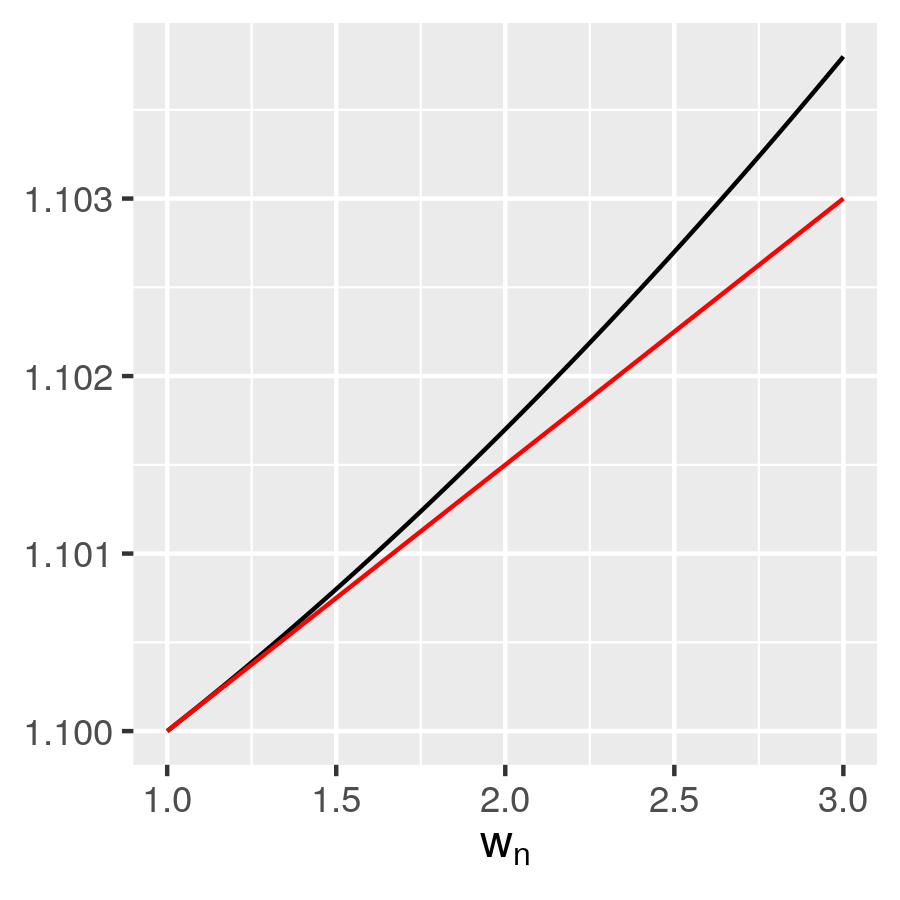
\includegraphics[width=0.98\textwidth]{static_figures/weight_slope}
            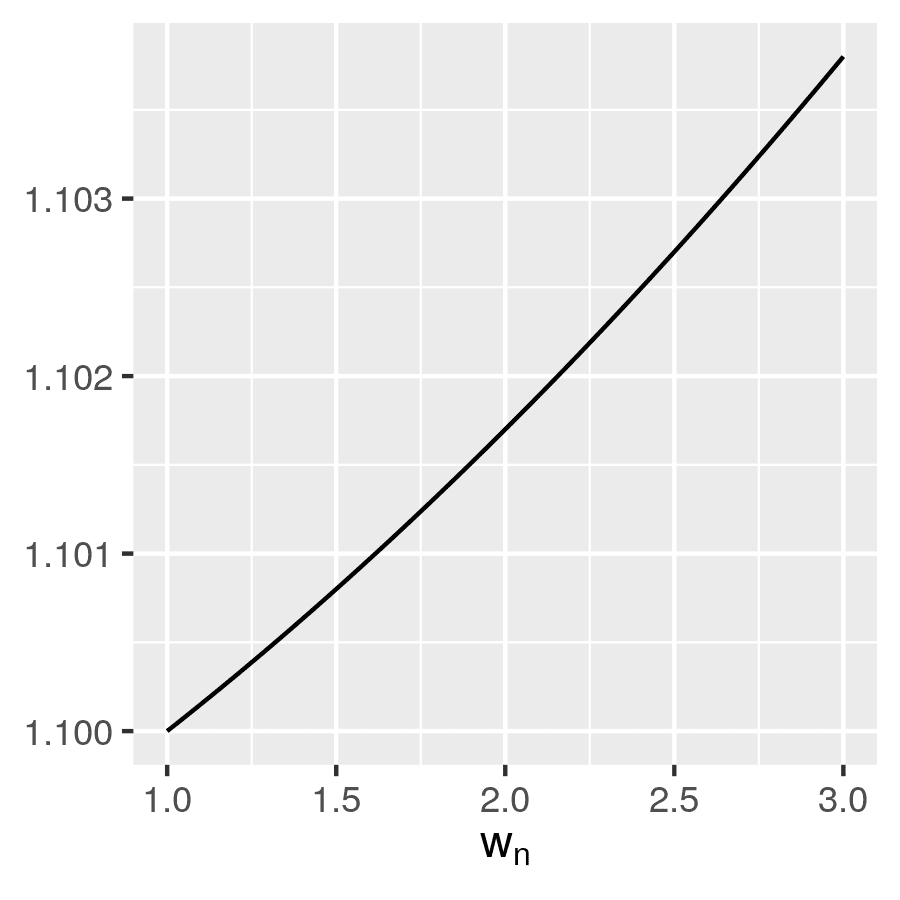
\includegraphics[width=0.98\textwidth]{static_figures/e_beta_w}
        };
        % \onslide<5-> {
        % \begin{scope}[x={(image.south east)},y={(image.north west)}]
        %     \draw[] (0.2,0.5)
        %             node[above,black,fill=white]
        %             {\small $\expect{p(\theta \vert \x, \w)}{\theta}$};
        % \end{scope}
        % }
        }
        \onslide<1->{
        \begin{scope}[x={(image.south east)},y={(image.north west)}]
            \draw[blue, thick, <-] (0.2,0.23) -- ++(0.1,0.25)
                    node[above,black,fill=white]
                    {\small $\thetafun(\thetahat)$};
        \end{scope}
        }
        \onslide<1->{
        \begin{scope}[x={(image.south east)},y={(image.north west)}]
            \draw[blue, thick, <-] (0.8,0.8) -- ++(-0.1,0.1)
                    node[left,black,fill=white]
                    {\small $\thetafun(\thetahat(\w))$};
        \end{scope}
        }
        \onslide<1->{
        \begin{scope}[x={(image.south east)},y={(image.north west)}]
            \draw[red, thick, -] (0.18,0.18) -- ++(1.2 * 0.6, 1.2 * 0.48);
        \end{scope}
        }
        \onslide<1->{
        \begin{scope}[x={(image.south east)},y={(image.north west)}]
            \draw[blue, thick, <-] (0.8,0.65) -- ++(0.02,-0.1)
                    node[below,black,fill=white]
                    {\small Slope $ = \infl_n$};
        \end{scope}
        }
    \end{tikzpicture}
%}
\end{minipage}

%
\begin{align*}
%
\thetafun(\thetahat(\w)) ={}&
\thetafun(\thetahat) + \sumn \infl_n (\w_n - 1) +
\textrm{Higher-order derivatives}
% \\
% \var{\w \sim \mathrm{Boot}}{\sqrt{N} \thetafun(\thetahat(\w))} \approx{}&
% \var{\w \sim \mathrm{Boot}}{\sumn \sqrt{N} \infl_n (\w_n - 1)} =
% \sumn N \infl_n^2 = \noise^2.
%
\end{align*}
%
\onslide<1->{
\vspace{-0.5em}
\textbf{Key idea: }
Controlling higher-order derivatives can control the error.
}
\end{frame}



%%%%%%%%%%%%%%%%%%%%%%%%%%%%%%%%%%%%%%%%%%%%%%%%%%%%%%%%%%%%%%%%%%%%%%%%%
%%%%%%%%%%%%%%%%%%%%%%%%%%%%%%%%%%%%%%%%%%%%%%%%%%%%%%%%%%%%%%%%%%%%%%%%%
%%%%%%%%%%%%%%%%%%%%%%%%%%%%%%%%%%%%%%%%%%%%%%%%%%%%%%%%%%%%%%%%%%%%%%%%%


\begin{frame}{The linear approximation.}
%
Let $W_\alpha$ be the set of weight vectors with no more than $\lfloor \alpha N
\rfloor$ zeros.

Let $H(\theta, \d_n) := \fracat{\partial G(\theta, \d_n)}{\partial
\theta^T}{\theta}$.

\begin{assu}
Fix the dataset.
Assume there exists a compact $\thetadom \subseteq \mathbb{R}^D$
with $\thetahat(\w) \in \thetadom$ for all $\w \in W_\alpha$.
Assume that, for all $\theta \in \thetadom$:
%
\begin{itemize}
    \item $\meann H(\theta, \d_n)$ and $\meann G(\theta, \d_n)$ are bounded.
    \item $\meann H(\theta, \d_n)$ is uniformly non-singular and
    Lipschitz (in $\theta$).
    \item $\thetafun(\theta)$ has a Lipschitz first derivative.
\end{itemize}
%
\end{assu}

%
\begin{theorem}
%
For sufficiently small $\alpha$, under the above assumption,
%
\begin{align*}
%
\sup_{\w \in W_\alpha} \abs{\thetafunlin(\w) - \thetafun(\thetahat(\w))}
    \le{}& C_1 \alpha \textrm{ and }
\sup_{\w \in W_\alpha} \abs{\thetafun(\thetahat(\w)) - \thetafun(\thetahat)}
    \le{} C_2 \sqrt{\alpha}.
%
\end{align*}
%
where $C_1$ and $C_2$ are given by the quantities in the assumption.
%
\end{theorem}

\end{frame}
